% A simple template for LaTeX documents
% 
% To produce pdf run:
%   $ pdflatex paper.tex 
%

\documentclass[12pt]{article}

% Begin paragraphs with new line
\usepackage{parskip}  

% Change margin size
\usepackage[margin=1in]{geometry}   

% Graphics Example:  (PDF's make for good plots)
\usepackage{graphicx}               
% \centerline{\includegraphics{figure.pdf}}

% Allows hyperlinks
\usepackage{hyperref}

% Blocks of code
\usepackage{listings}
\lstset{basicstyle=\ttfamily, title=\lstname}
% Insert code like this. replace `plot.R` with file name.
% \lstinputlisting{plot.R}

% Supports proof environment
\usepackage{amsthm}

% Allows writing \implies and align*
\usepackage{amsmath}

% Allows mathbb{R}
\usepackage{amsfonts}


%%%%%%%%%%%%%%%%%%%%%%%%%%%%%%%%%%%%%%%%%%%%%%%%%%%%%%%%%%%%
\begin{document}

\title{US Korea Exchange Rates \\ STA206 Final Project}
\date{December 15, 2014}
\author{Clark Fitzgerald clarkfitzg@gmail.com \\ 
        Amy Kim atykim@ucdavis.edu}

\maketitle

\begin{abstract}
    We analyze the exchange rate between the United States and South Korea
    (hereafter Korea) using monthly country level economic data.
\end{abstract}

\section{Introduction}

\subsection{Background}

In today's highly connected global society people and money move between
countries. The exchange rates between countries determine the value of
that currency.

We analyze data on exchange rate between the US and Korea from 1999 to
2014. In 1997 the IMF crisis in Korea perturbed the economic indicators,
but in looking at the data we can see that it has been stable since 1999.

\subsection{Questions}

\begin{enumerate}

    \item How do exchange rates behave?

    \item Can we predict the exchange rate between two countries?  

    \item When is the best time to exchange currency from won (Korean
        currency) to dollar or vice versa?  

    \item Can we find a linear relationship
        that can be applied over other countries' currency? 

\end{enumerate}

\subsection{Motivation}

Sometimes it's necessary to transfer funds between countries. This is true
for both individuals, families, and organizations. The exchange rate can
vary substantially over time. For example, in
Figure~\ref{fig:exchange_rate} we observe the exchange rate between Korea
and the US varying between 900 and 1400 Korean Won per US Dollar. A quick
calculation on this data 
implies that during this period a fixed amount of Korean currency 
could have been worth \$100,000 or \$158,000, depending on when it was  
exchanged. 

Hence if one has a significant amount of capital to move from
one country to another and some flexibility around the timing then it makes
sense to do it when the exchange rates
are favorable for the transfer. For example, you may want to sell a
house in Korea and put that money towards a house in the US.

If one plans to go on vacation in a foreign country then it makes sense to
visit a country where the exchange rate is favorable.

\subsection{Data}
We use data from Quandl.com, a service that provides clean, documented
data from a wide variety of sources including the US Federal Reserve,
World Bank, and the National Bank of Korea. 
{\tt Exchange rate} between Korean Won and US dollar is the primary $Y$
variable.

For each country we will examine the following variables:

\begin{itemize}
    \item {\tt gdp} The gross domestic product. Units: USD Million
    \item {\tt unemployment rate} The percentage of the labor force who are unemployed and actively seeking work. Units: Percent (monthly)
    \item {\tt exports} The total value of the goods and services
produced domestically and purchased by foreign entities. Units: USD Million (Monthly)
    \item {\tt imports} The total value of a country's imports of physical goods and payments to foreigners for services like shipping and tourism. Units: USD Million (Monthly)
    \item {\tt interest rate} The monthly average of the central bank policy rate. This is the interest rate the central bank charges on loans to commercial banks. Units: Percent (Monthly)
    \item {\tt inflation rate} The growth rate of the prices. (Monthly)
    \item {\tt consumer produce index} The Consumer Price Index (CPI) is a measure of inflation related to the cost of living. Units: Index Points 2010=100, NSA (Monthly)
    \item {\tt debt} The total amount of public and private debt owned by foreign creditors. Units: USD Million Current Prices, NSA (quarterly)
    \item {\tt gdp deflator} The relative difference between the real and nominal GDPs. Units: Index Points NSA
    \item {\tt goverment spending} The yearly expenditure of the federal
        government. Units: local currency
    \item {\tt political party} Categorical variable for the political
party of the president.
\end{itemize}

\section{Methods and Results}

\subsection{Data Collection}
The data is loaded directly using a
web API (Application programming interface).
Using this service will make it easier to repeat the analysis in the future, or conduct similar analyses between
different countries.



Figure~\ref{fig:correlation} shows a histogram of all the pairwise sample
correlations.

Figure~\ref{fig:na_plot_KOR} shows the variables which were interpolated.

Attempting to reference \cite{lamport94}.

\section{Conclusions and Discussion}


\newpage
\section{Appendix}

\listoffigures

\begin{figure}
  \centering
    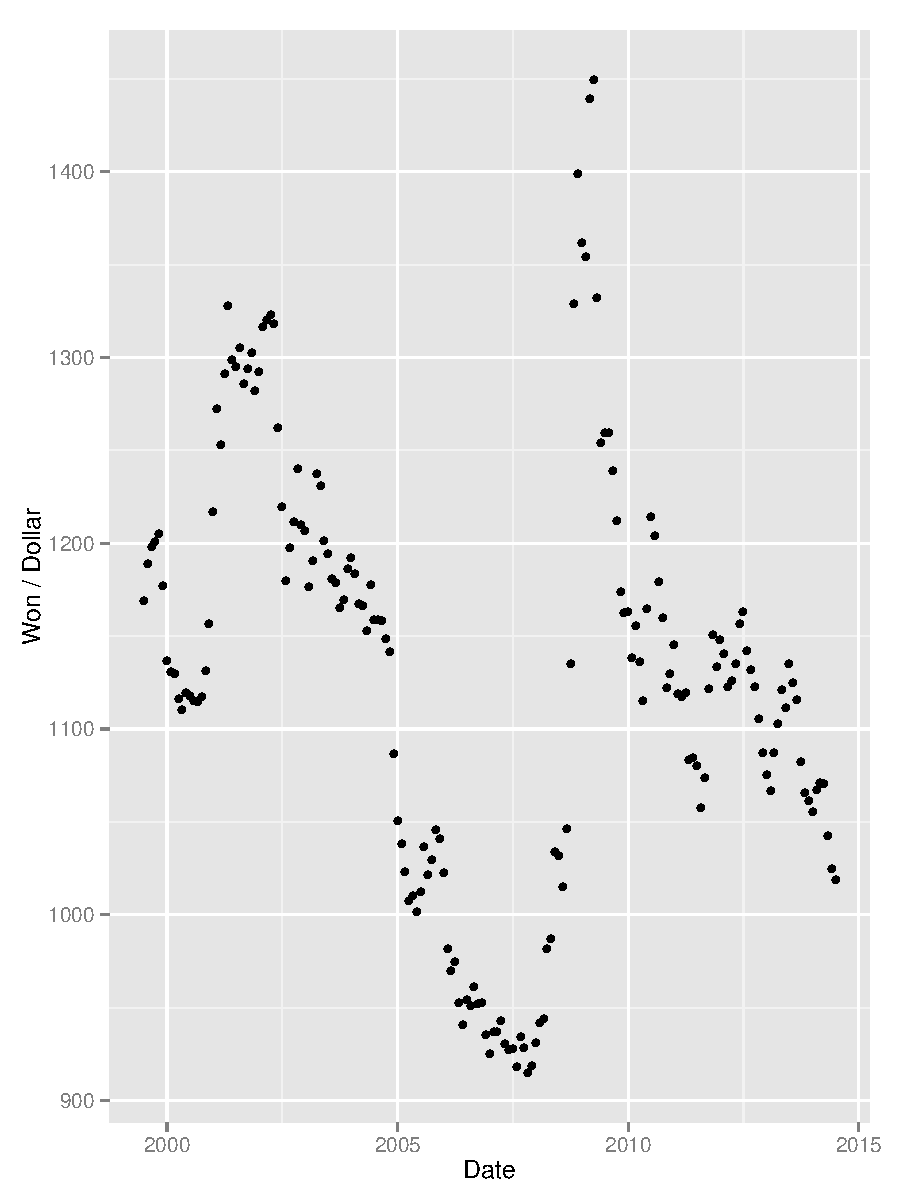
\includegraphics{exchange_rate.pdf}
  \caption{Exchange rate between US and South Korea from 1999 to 2014}
  \label{fig:exchange_rate}
\end{figure}

\begin{figure}
  \centering
    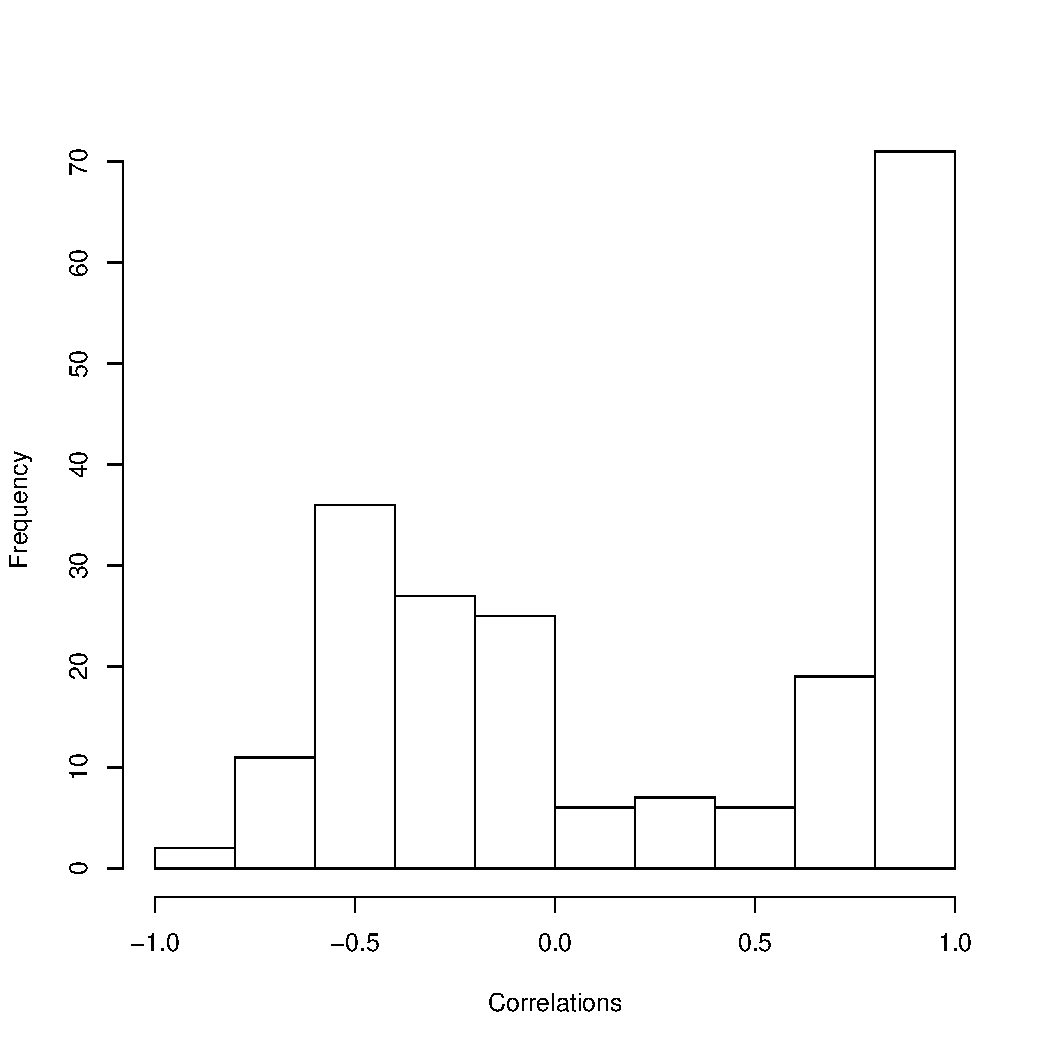
\includegraphics{correlation.pdf}
  \caption{Histogram of all pairwise sample correlations}
  \label{fig:correlation}
\end{figure}

\begin{figure}
  \centering
    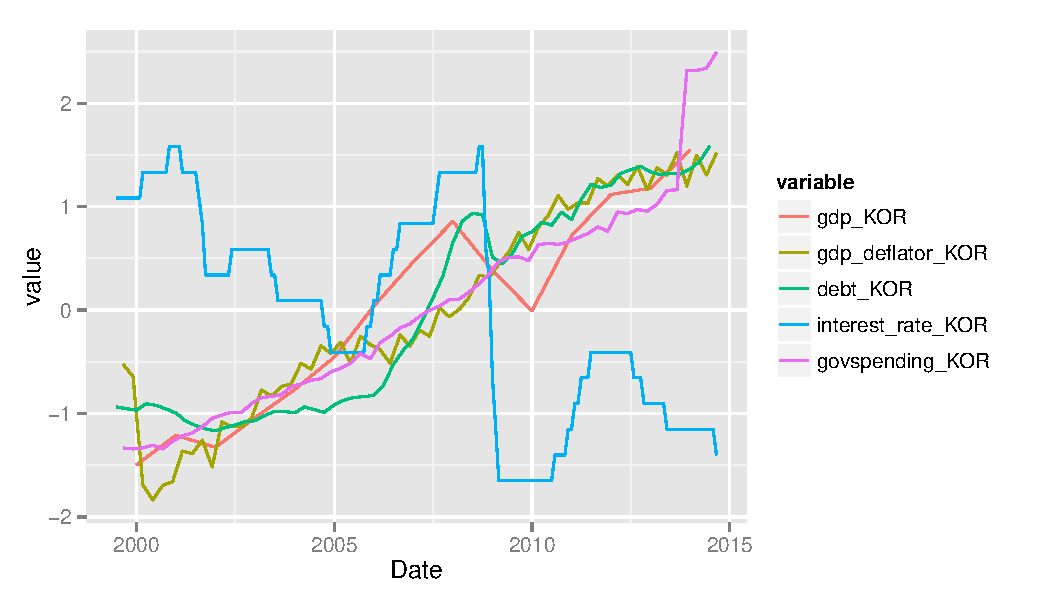
\includegraphics{na_plot_KOR.pdf}
  \caption{Scaled variables with NA values}
  \label{fig:na_plot_KOR}
\end{figure}

\newpage

\begin{thebibliography}{9}

\bibitem{lamport94}
  Leslie Lamport,
  \emph{\LaTeX: a document preparation system}.
  Addison Wesley, Massachusetts,
  2nd edition,
  1994.

\end{thebibliography}

\end{document}
